\section{Exercise B}

From the inference, we can state the following state:

\begin{itemize}
\item
p: Per moves his bishop
\item
r: Ren\'e moves his rook 
\item
d: Per moves his queen
\item
b: Ren\'e breaks the chessboard
\end{itemize}

The inference becomes:

\begin{center}
$ p \to b $ \\
$ r \leftrightarrow d $ \\
$ \neg d \land \neg p $ \\
\noindent\rule{2.5cm}{0.4pt} \\
$ d \to (r \land b) $ \\
\end{center}

\newpage

Using the tableau method, we get the following:

\begin{center}
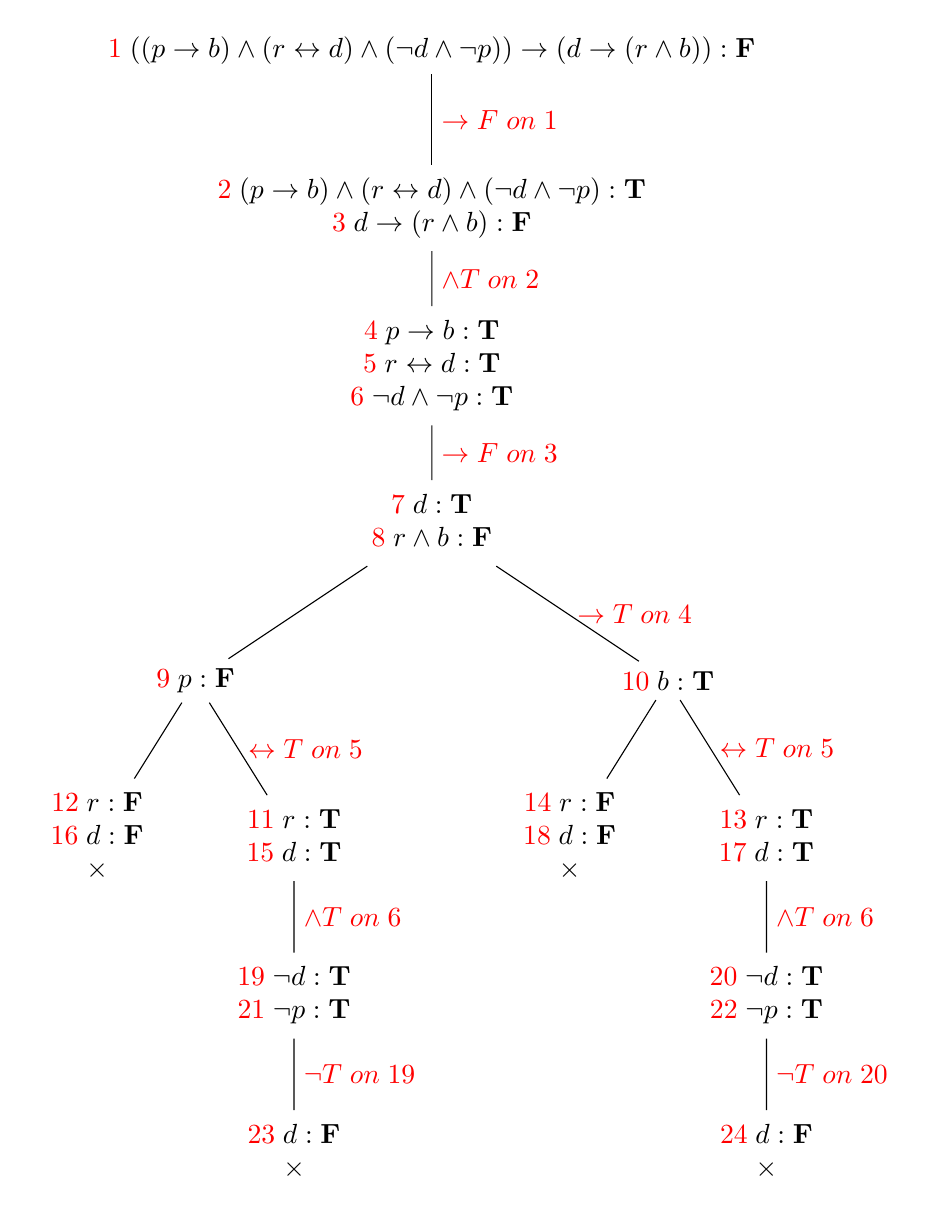
\begin{tikzpicture}

\node {$ \textcolor{red}{1}\; ((p \to b) \land (r \leftrightarrow d) \land (\neg d \land \neg p)) \to (d \to (r \land b)):\textbf{F} $} [sibling distance = 2cm] [level distance=20mm] 
        child {node {$ \begin{array}{c} \textcolor{red}{2}\; (p \to b) \land (r \leftrightarrow d) \land (\neg d \land \neg p):\textbf{T} \\ \textcolor{red}{3}\; d \to (r \land b):\textbf{F} \end{array} $} 
            child {node {$ \begin{array}{c} \textcolor{red}{4}\; p \to b:\textbf{T} \\ \textcolor{red}{5}\; r \leftrightarrow d:\textbf{T} \\ \textcolor{red}{6}\; \neg d \land \neg p:\textbf{T} \end{array} $}
                child {node {$ \begin{array}{c} \textcolor{red}{7}\; d:\textbf{T} \\ \textcolor{red}{8}\; r \land b:\textbf{F} \end{array} $} [sibling distance = 6cm]
                    child {node {$ \textcolor{red}{9}\; p:\textbf{F} $} [sibling distance = 2.5cm]
                        child {node {$ \begin{array}{c} \textcolor{red}{12}\; r:\textbf{F} \\ \textcolor{red}{16}\; d:\textbf{F} \\ \times \end{array} $}}
                        child {node {$ \begin{array}{c} \textcolor{red}{11}\; r:\textbf{T} \\ \textcolor{red}{15}\; d:\textbf{T}\end{array} $}
                        child {node {$ \begin{array}{c} \textcolor{red}{19}\; \neg d:\textbf{T} \\ \textcolor{red}{21}\; \neg p:\textbf{T}\end{array} $}
                        child {node {$ \begin{array}{c} \textcolor{red}{23}\; d:\textbf{F} \\ \times \end{array} $}
                        edge from parent node [right, red] {$\neg T\;on\; 19$}}
                        edge from parent node [right, red] {$\land T\;on\; 6$}}
                        edge from parent node [right, red] {$\leftrightarrow T\;on\; 5$}}}
                    child {node {$ \textcolor{red}{10}\; b:\textbf{T} $} [sibling distance = 2.5cm]
                        child {node {$ \begin{array}{c} \textcolor{red}{14}\; r:\textbf{F} \\ \textcolor{red}{18}\; d:\textbf{F} \\ \times \end{array} $}}
                        child {node {$ \begin{array}{c} \textcolor{red}{13}\; r:\textbf{T} \\ \textcolor{red}{17}\; d:\textbf{T}\end{array} $}
                        child {node {$ \begin{array}{c} \textcolor{red}{20}\; \neg d:\textbf{T} \\ \textcolor{red}{22}\; \neg p:\textbf{T}\end{array} $}
                        child {node {$ \begin{array}{c} \textcolor{red}{24}\; d:\textbf{F} \\ \times \end{array} $}
                        edge from parent node [right, red] {$\neg T\;on\; 20$}}
                        edge from parent node [right, red] {$\land T\;on\; 6$}}
                        edge from parent node [right, red] {$\leftrightarrow T\;on\; 5$}}
                        edge from parent node [right, red] {$\to T\;on\; 4$}}
                        edge from parent node [right, red] {$\to F\;on\; 3$}}
                        edge from parent node [right, red] {$\land T\;on\; 2$}} 
                        edge from parent node [right, red] {$\to F\;on\; 1$}};

\end{tikzpicture}
\end{center}

There is no truth assignment that makes the formula false, thus it is \underline{valid} and the inference is logically correct.